\section{Experiments}
\begin{figure}
  \centering
  \begin{subfigure}[b]{0.48\linewidth}
    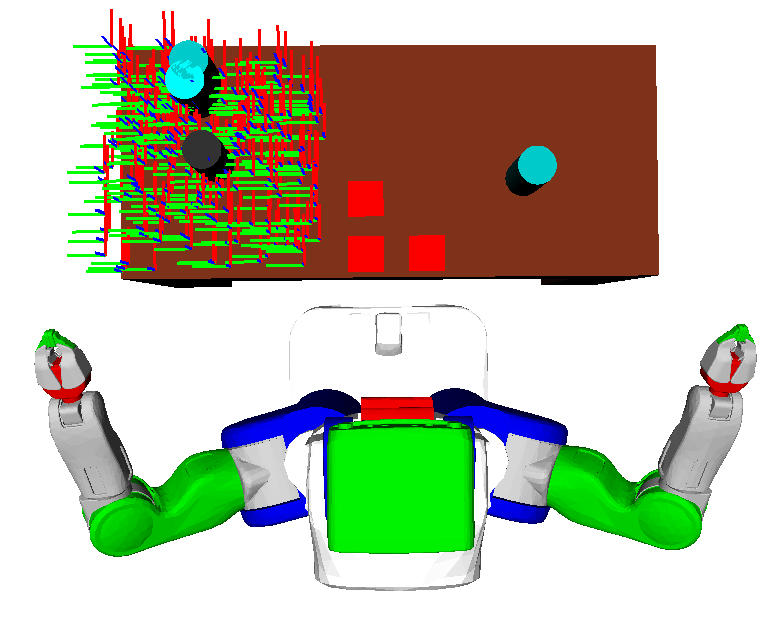
\includegraphics[width=\textwidth]{images/learngs.png}
    \caption{Initial distribution}
  \end{subfigure}
  \begin{subfigure}[b]{0.48\linewidth}
    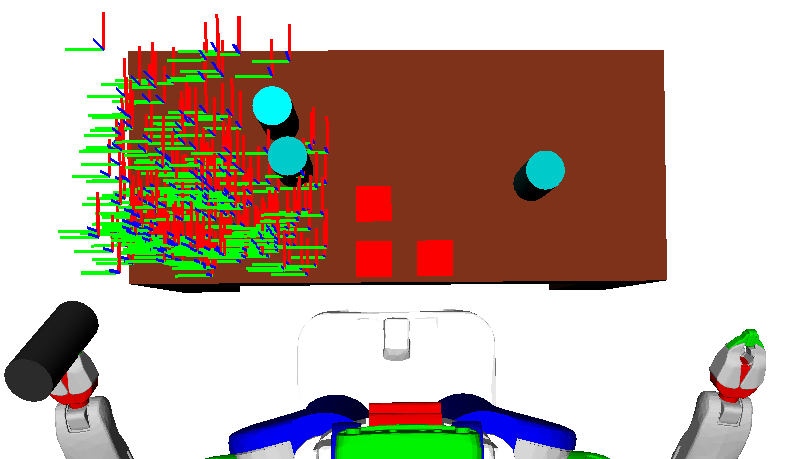
\includegraphics[width=\textwidth]{images/learng5.png}
    \caption{After 5 iterations.}
  \end{subfigure}
  \begin{subfigure}[b]{0.48\linewidth}
    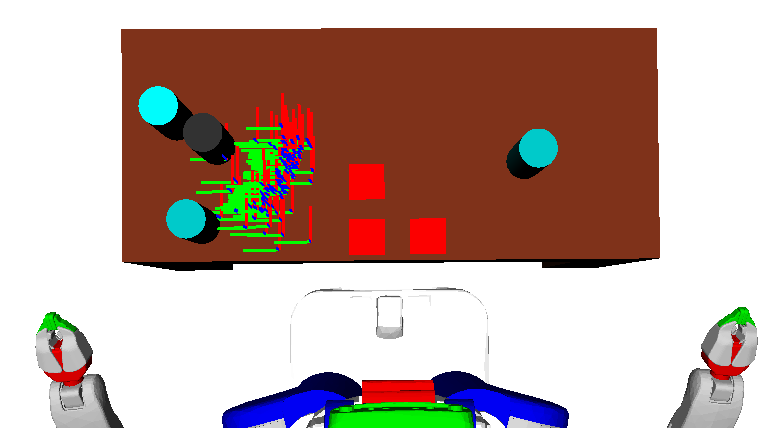
\includegraphics[width=\textwidth]{images/learng15.png}
    \caption{After 15 iterations.}
  \end{subfigure}
  \begin{subfigure}[b]{0.48\linewidth}
    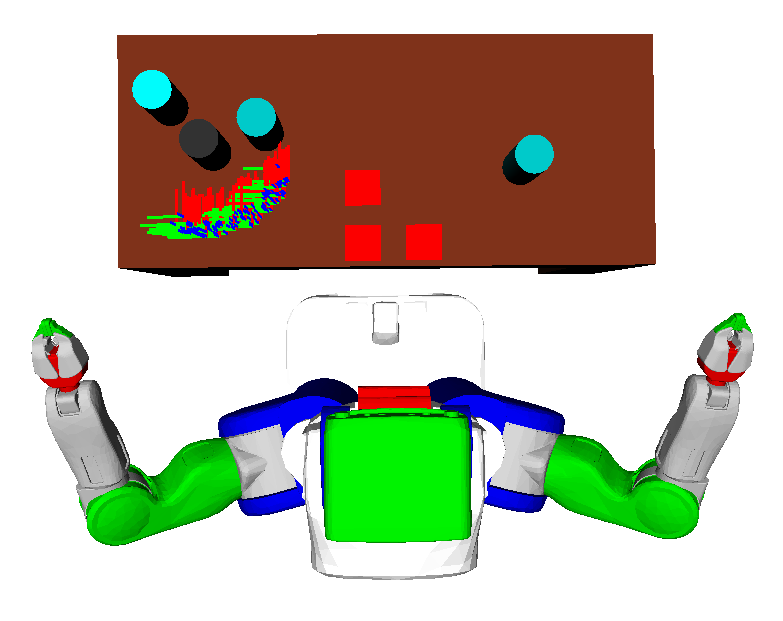
\includegraphics[width=\textwidth]{images/learng20.png}
    \caption{Final distribution.}
  \end{subfigure}
  \caption{Learned left arm grasping distributions used to
pick up the black can, after different training iterations.
An iteration refers to a single run of randomized refinement,
which terminates after $L$ calls to the resample function. The
initial distribution is uniform because we initialize weights to $\vec{\mathbf{0}}$.
The final distribution is after 20 iterations.}
  \label{fig:training}
\end{figure}

\begin{figure}
  \centering
  \begin{subfigure}[b]{0.3\linewidth}
    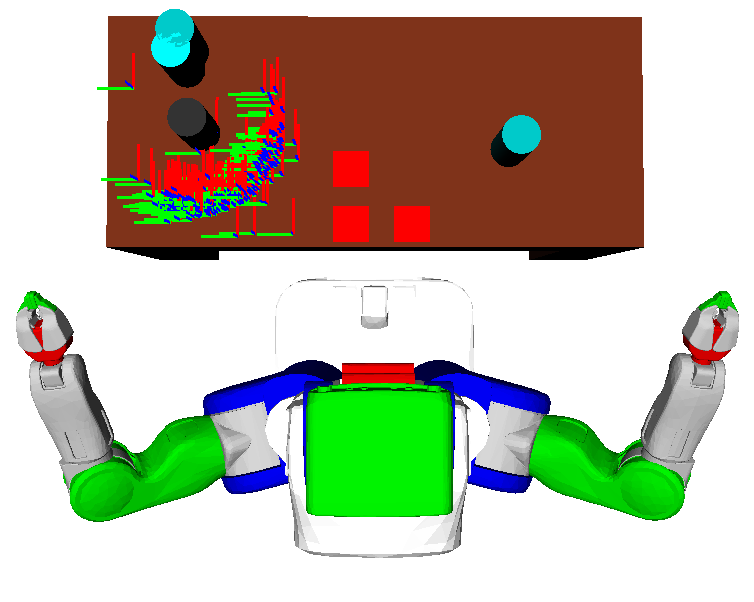
\includegraphics[width=\textwidth]{images/finalgraspnoobstr.png}
    \caption{}
  \end{subfigure}
  \begin{subfigure}[b]{0.3\linewidth}
    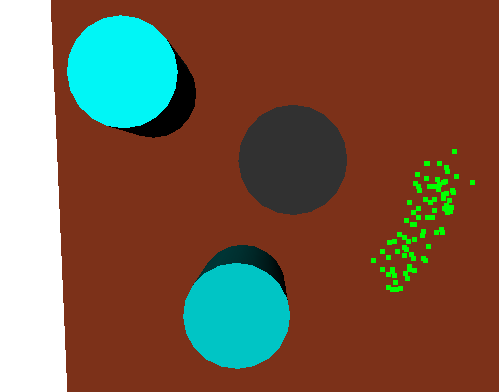
\includegraphics[width=\textwidth]{images/finalgraspobstr.png}
    \caption{}
  \end{subfigure}
  \begin{subfigure}[b]{0.3\linewidth}
    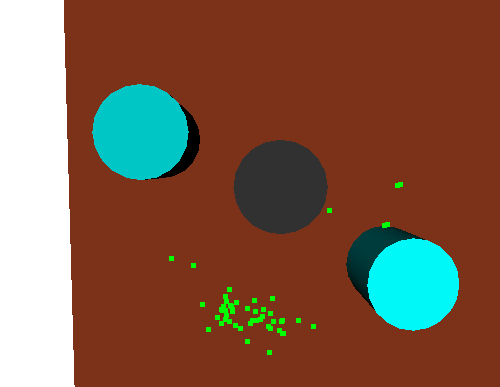
\includegraphics[width=\textwidth]{images/finalgraspobstr2.png}
    \caption{}
  \end{subfigure}
  \caption{The final distribution from \figref{fig:training}
is shown with different obstruction layouts. The system learns to
avoid obstructions while providing a good set of grasping poses.}
  \label{fig:obstr}
\end{figure}

\begin{table}
  \centering
  \vspace{8pt}
  \tabcolsep=0.11cm{
  \begin{tabular}{ccccc}
    \toprule[1.5pt]
      \textbf{System} & \textbf{Scenario} & \textbf{\% Solved} & \textbf{Avg MP Time (s)} & \textbf{Avg \# MP Calls}\\
    \midrule[2pt]
      B & 1 & 100 & 8.16 & 18.93\\
    \midrule
      L & 1 & 96 & 6.11 & 11.5\\
    \midrule[1.5pt]
      B & 2 & 96 & 8.74 & 19.7\\
    \midrule
      L & 2 & 94 & 12.26 & 20.77\\
    \midrule[1.5pt]
      B & 3 & 84.44 & 10.77 & 23.16\\
    \midrule
      L & 3 & 97.78 & 10.6 & 19.1\\
    \midrule[1.5pt]
      B & 4 & 33.33 & 12.1 & 21.1\\
    \midrule
      L & 4 & 96.67 & 9.19 & 17.78\\
    \midrule[1.5pt]
      B & 5 & 100 & 4.52 & 12.24\\
    \midrule
      L & 5 & 100 & 5.94 & 15.36\\
    \bottomrule[1.5pt]
  \end{tabular}}
  \caption{Percent solved, along with time spent motion planning and number of calls to the motion
planner for the final refinement. Results are averaged across 50 test environments per scenario, when both
the baseline and our system succeed. The test environments
were grouped into batches of 5, and each batch first received independent training with a distinct random seed. For each scenario,
we provide baseline system results using hand-tuned sampling distributions (B) and results from running
our reinforcement learning system (L).}
  \label{table:results}
\end{table}

\subsection{Evaluation}
We evaluate our reinforcement learning system in several pick-and-place
tasks, varying the number of obstructions, obstruction locations, and whether
the base is allowed to move. We compare performance with that of the
hand-coded sampling distributions used in Srivastava et al.~\cite{srivastava2014combined}.
Because our learned distributions are optimized for producing motion planning
feasible samples, we do not evaluate performance on total system
running time; rather, we evaluate the refinement of only the final high level
plan. This is because, if we have a high level plan with \emph{no} valid refinement,
our system may find more IK-feasible samples (and thus trigger more calls to
the motion planner) than the baseline system. This causes increased time spent
on refinement attempts before raising error information back to the task planner,
which should not be penalized. The error propagation occurs when the iteration
limit is reached in the randomized refinement algorithm.

We use the reward function described earlier. Our weight
vectors are initialized to $\vec{\mathbf{0}}$ for all pose parameter types: grasp pose
for each arm, putdown pose for each arm, and base motion.
The initialization represents a uniform distribution across the limits of the geometric search space.
For grasp and putdown actions, the limits are a cube of side length 30 centimeters
around the target object or putdown location. For base motion actions, the limits are a
square of side length 1 meter around the object or location which the robot is approaching.
Currently, our feature function $f$ incorporates only geometric aspects of the sample and environment,
such as distance between the sample and object being grasped, and distance from the sample to
nearby obstructions.

Our experiments are conducted in Python 2.7 using the OpenRave simulator~\cite{Diankov_2008_6117} with a PR2 robot.
The motion planner we use is trajopt~\cite{schulman2013finding}, and the task planner is Fast-Forward~\cite{FF}.
The experiments were carried out in series on an Intel Core i7-4770K machine
with 16GB RAM.

We train and test five different scenarios, all of which share a common goal of
grasping a target object from a table and putting it down at a specific location on the table:
\begin{tightlist}
\item[\textbf{Scenario 1}:] Target object is surrounded by 1 obstruction.
\item[\textbf{Scenario 2}:] Target object is surrounded by 2 obstructions.
\item[\textbf{Scenario 3}:] Target object is surrounded by 3 obstructions.
\item[\textbf{Scenario 4}:] Target object is surrounded by 1 obstruction,
and putdown location is obstructed in cardinal directions.
\item[\textbf{Scenario 5}:] Target object is surrounded by 1 obstruction,
but the robot begins out of reach of the table and must learn base motion.
\end{tightlist}

For the first 4 scenarios, we use $N = 20$, $L = 16$, and $\epsilon = 4$.
For the final one involving base motion, we use $N = 60$, $L = 100$, and $\epsilon = 20$,
allowing randomized refinement to run for more iterations because the high level plan
is longer. The locations of the obstructions surrounding the target object were
sampled uniformly from a thick ring around the object with inner radius 0.13 meters
and outer radius 0.25 meters. Table \ref{table:results} summarizes our quantitative results.
\figref{fig:cover} plots learned distributions for a move-grasp-move-putdown sequence of actions.
\figref{fig:training} illustrates the training of a grasp distribution, and \figref{fig:obstr}
shows how the learned distribution interacts with obstructions.

\subsection{Discussion}
The quantitative results indicate that our system performs comparably to
the baseline in all five environment setups. Scenario 4, for which our learning
algorithm greatly outperforms, was designed to
be difficult for the baseline system, because the putdown pose sample space
is discretized such that the gripper always approaches the putdown location from a
cardinal direction. These cardinal directions were blocked by obstructions,
meaning the baseline system will generally perform poorly in this environment,
illuminating its lack of robustness.